\documentclass[conference]{IEEEtran}

% ---------------------------------------------------------------
% Packages
% ---------------------------------------------------------------
\usepackage{cite}
\usepackage{amsmath,amssymb,amsfonts}
\usepackage{algorithmic}
\usepackage{graphicx}
\usepackage{textcomp}
\usepackage{xcolor}
\usepackage{booktabs}
\usepackage{multirow}
\usepackage{url}
\usepackage{hyperref}
\usepackage{pdfpages}

\hypersetup{
    colorlinks=false,
    pdfborder={0 0 0}
}

% ---------------------------------------------------------------
% Document
% ---------------------------------------------------------------
\begin{document}

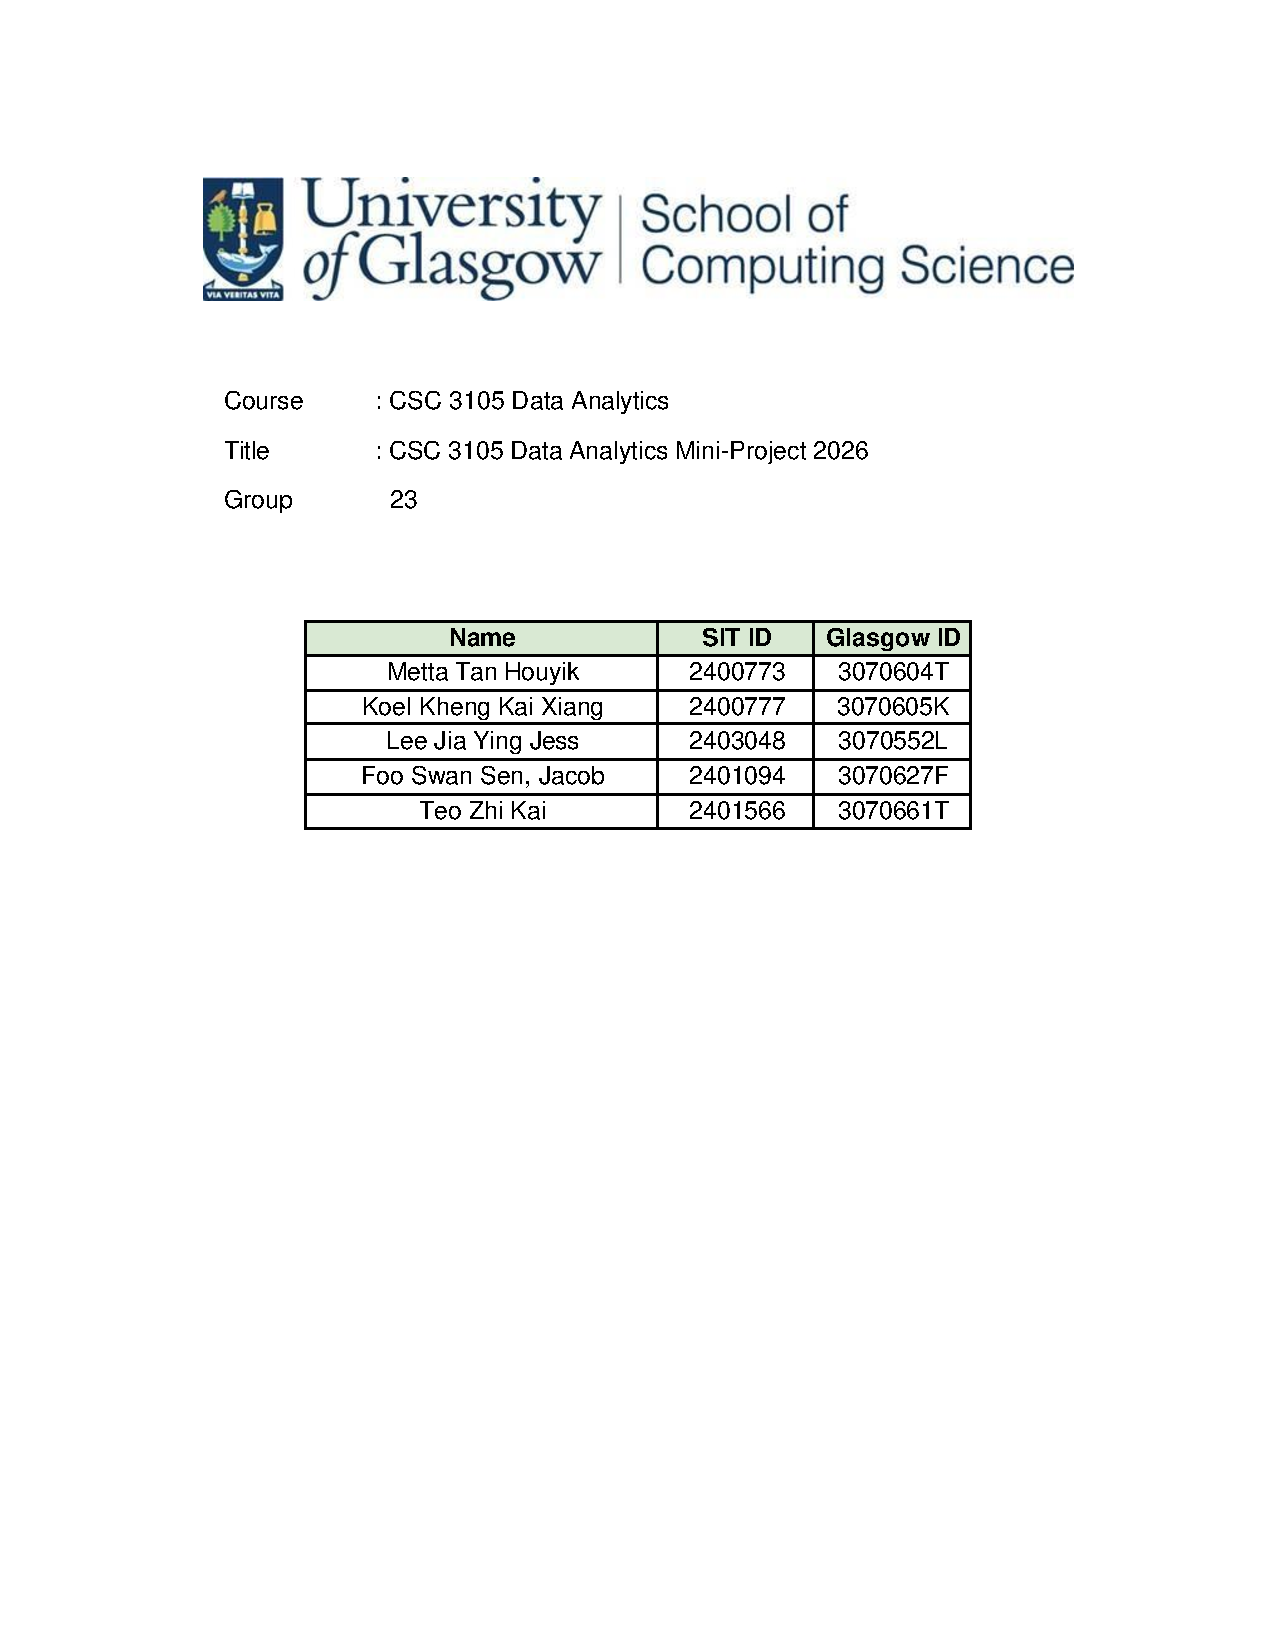
\includepdf[pages=1]{cover.pdf}

% ---------------------------------------------------------------
% ABSTRACT
% ---------------------------------------------------------------
\begin{abstract}
Precise indoor localisation is a critical enabling technology for autonomous vehicles,
drone navigation, asset tracking, and smart building systems. Global Positioning System
(GPS) signals cannot penetrate building structures reliably, and conventional Radio
Frequency (RF) approaches suffer from severe measurement bias under
Non-Line-of-Sight (NLOS) multipath conditions. This paper presents a complete
data-analytics pipeline that classifies Ultra-Wideband (UWB) Channel Impulse Response
(CIR) measurements as Line-of-Sight (LOS) or NLOS and simultaneously estimates the
true ranging distance for two dominant propagation paths. Using a real empirical dataset
of 42{,}000 samples collected from seven distinct indoor environments with a Decawave
DWM1000 module (Apple/Qorvo UWB vendor), we apply the three-stage Data Analytics
process: Data Preparation, Data Mining, and Data Visualisation. After CIR normalisation
by the received preamble accumulation count (\texttt{RXPACC}) and feature-importance
ranking via Random Forest, nine features are selected for a Random Forest Classifier
trained on an 80:20 train/test split. Path 1 (primary) LOS/NLOS classification achieves
a test accuracy of \textbf{91.40\%}. Separate Random Forest Regressors estimate the
measured range for Path 1 (RMSE = 1.5027\,m, $R^{2}$ = 0.5921) and for Path 2
(RMSE = 1.7823\,m), a secondary reflected path extracted from the CIR profile.
Results demonstrate that ensemble tree methods can effectively exploit UWB signal
statistics to support robust, infrastructure-light indoor positioning.
\end{abstract}

\begin{IEEEkeywords}
UWB, LOS, NLOS, channel impulse response, indoor localisation, Random Forest,
ranging error, classification, regression.
\end{IEEEkeywords}

% ---------------------------------------------------------------
% I. INTRODUCTION / LITERATURE REVIEW
% ---------------------------------------------------------------
\section{Introduction and Literature Review}

\subsection{Indoor Positioning and the Limits of GPS}
Precise localisation underpins a wide class of modern applications: warehouse robotics,
hospital asset tracking, pedestrian navigation inside malls or airports, autonomous drones,
and emerging Industry 4.0 manufacturing cells \cite{zafari2019survey}. The dominant
outdoor solution, GPS, relies on unobstructed line-of-sight links to multiple satellites.
Building materials---reinforced concrete, metallic partitions, low-energy glass---attenuate
satellite signals by 20--40\,dB, making sub-metre indoor positioning impossible with GPS
alone \cite{liu2007survey}. Alternative RF technologies have therefore been explored:
Wi-Fi (IEEE 802.11) fingerprinting offers 2--5\,m accuracy but is highly sensitive to
environmental change; Bluetooth Low Energy beacons suffer similar accuracy limitations;
5G positioning is promising but infrastructure-heavy.

\subsection{Ultra-Wideband for Indoor Ranging}
Ultra-Wideband (UWB) operates across a spectrum of 3.1--10.6\,GHz with an instantaneous
bandwidth exceeding 500\,MHz, enabling time-of-flight (ToF) ranging with centimetre-level
resolution under ideal LOS conditions \cite{gezici2005localization}. The Decawave
DWM1000 chip (now supplied by Qorvo, adopted by Apple for AirTag and iPhone spatial
awareness) implements IEEE 802.15.4a UWB and reports a rich set of diagnostic registers
alongside the raw CIR vector containing 1\,016 complex magnitude samples at 1\,ns
resolution. Under LOS conditions the CIR exhibits a sharp, dominant first peak; under
NLOS conditions walls and furniture cause multipath components that obscure or delay
the first arrival, biasing ToF estimates and introducing ranging errors of several metres
(see Fig.~2 of the project brief) \cite{wymeersch2012machine}.

\subsection{The LOS/NLOS Challenge}
When the direct path between a UWB anchor and tag is blocked, the measured range
(\texttt{RANGE}) systematically over-estimates the true distance because the signal
travels a longer reflected or diffracted path. This positive bias---sometimes exceeding
5\,m in furnished offices---degrades trilateration or hyperbolic positioning accuracy
severely. State-of-the-art mitigation strategies fall into three categories:
\begin{itemize}
    \item \textbf{Geometric/statistical methods}: threshold-based first-path detection,
          hypothesis testing on receive signal strength \cite{guvenc2009survey}.
    \item \textbf{Channel-feature machine learning}: SVMs, k-NN, and neural networks
          trained on hand-crafted CIR statistics \cite{maranò2010nlos}.
    \item \textbf{Deep learning on raw CIR}: CNNs applied directly to the full
          1\,016-sample CIR vector \cite{bregar2018improving}.
\end{itemize}

Bregar and Mo\v{z}ina \cite{bregar2018improving} published the dataset used in this work
and demonstrated that a multi-layer perceptron (MLP) trained on statistical CIR features
outperforms threshold heuristics. However, deep CNN approaches on raw CIR require
substantial compute and are opaque. Our work differs in three ways: (i) we perform
explicit feature-importance ranking to reduce the 1\,016-dimensional CIR to nine
interpretable features; (ii) we use an ensemble Random Forest that is inherently
interpretable and robust to outliers; and (iii) we extend the pipeline to a two-path
framework, extracting and estimating the second dominant propagation path directly
from the CIR profile, providing a richer signal model for downstream positioning.

% ---------------------------------------------------------------
% II. PROPOSED SOLUTION
% ---------------------------------------------------------------
\section{Proposed Solution}

Our solution follows the three-stage \textbf{3D Process of Data Analytics}: Data
Preparation (1st D), Data Mining (2nd D), and Data Visualisation (3rd D). The full
pipeline is implemented in a single Jupyter notebook
(\texttt{code/CSC3105\_Main\_Pipeline.ipynb}) supported by helper modules
(\texttt{dataprep.py}, \texttt{datamining.py}, \texttt{uwb\_dataset.py}).

\subsection{Data Preparation (1st D)}

\subsubsection{Dataset Description}
The UWB-LOS-NLOS dataset \cite{bregar2018improving} consists of seven CSV files
(\texttt{uwb\_dataset\_part1.csv} through \texttt{uwb\_dataset\_part7.csv}), each
corresponding to one indoor environment: Office~1, Office~2, Small Apartment, Small
Workshop, Kitchen with Living Room, Bedroom, and Boiler Room. Each environment
provides 3{,}000 LOS and 3{,}000 NLOS samples, yielding a balanced total of
21{,}000 LOS and 21{,}000 NLOS samples (42{,}000 overall). Each row contains 1\,032
columns: 15 diagnostic features, the ground-truth label (\texttt{NLOS}: 0 = LOS,
1 = NLOS), one measured-range column (\texttt{RANGE}/\texttt{Measured\_range}), and
1\,016 CIR magnitude samples (\texttt{CIR0}--\texttt{CIR1015}).

\subsubsection{Data Cleaning}
All seven CSV files are loaded with \texttt{pandas.read\_csv} and concatenated into a
single dataframe using \texttt{pd.concat(all\_frames, ignore\_index=True)}. The first
processing step strips trailing whitespace from all column headers
(\texttt{df.columns.str.strip()}) to prevent key-errors during indexing. Column names
are subsequently hard-reset to a standard ordered list:

\begin{verbatim}
standard_headers = [
 'NLOS', 'Measured_range', 'FP_IDX',
 'FP_AMP1', 'FP_AMP2', 'FP_AMP3',
 'STDEV_NOISE', 'CIR_PWR', 'MAX_NOISE',
 'RXPACC', 'CH', 'FRAME_LEN',
 'PREAM_LEN', 'BITRATE', 'PRFR']
\end{verbatim}

\subsubsection{CIR Normalisation}
Raw CIR values are reported as 16-bit integers accumulated over the preamble period.
The accumulation count is stored in the \texttt{RXPACC} register. Normalising by
\texttt{RXPACC} removes the receiver-gain dependency:
\begin{equation}
  \hat{c}_{k} = \frac{c_{k}}{\max(\texttt{RXPACC},\, 1)}, \quad k = 0,\ldots,1015
\end{equation}
This is applied column-wise: \texttt{df[cir\_cols] = df[cir\_cols].div(df['RXPACC']\\.replace(0,~1),~axis=0)}.

\subsubsection{Feature Importance Ranking}
With 1\,016 raw CIR dimensions, direct classification would be memory-intensive and
prone to the curse of dimensionality. We therefore train a preliminary
\texttt{RandomForestClassifier(n\_estimators=100, random\_state=42)} on 14 diagnostic
features to obtain Gini-impurity-based importance scores. The candidate features are:
\texttt{Measured\_range}, \texttt{FP\_IDX}, \texttt{FP\_AMP1}, \texttt{FP\_AMP2},
\texttt{FP\_AMP3}, \texttt{STDEV\_NOISE}, \texttt{CIR\_PWR}, \texttt{MAX\_NOISE},
\texttt{RXPACC}, \texttt{CH}, \texttt{FRAME\_LEN}, \texttt{PREAM\_LEN},
\texttt{BITRATE}, \texttt{PRFR}. Features with near-zero importance (configuration
constants such as \texttt{CH}, \texttt{FRAME\_LEN}, \texttt{PREAM\_LEN},
\texttt{BITRATE}, \texttt{PRFR}) are discarded, leaving nine predictive features:

\begin{center}
\small
\begin{tabular}{ll}
\toprule
\textbf{Feature} & \textbf{Meaning} \\
\midrule
\texttt{RXPACC}       & Preamble accumulation count \\
\texttt{CIR\_PWR}    & Channel impulse response power \\
\texttt{FP\_AMP3}    & First-path amplitude (3rd estimate) \\
\texttt{FP\_AMP2}    & First-path amplitude (2nd estimate) \\
\texttt{MAX\_NOISE}  & Maximum noise sample in CIR \\
\texttt{FP\_AMP1}    & First-path amplitude (1st estimate) \\
\texttt{STDEV\_NOISE}& Standard deviation of noise floor \\
\texttt{FP\_IDX}     & First-path index in CIR array \\
\texttt{Measured\_range} & Time-of-flight range estimate \\
\bottomrule
\end{tabular}
\end{center}

\subsubsection{Two-Path Framework}
A key design decision is the introduction of a two-path signal model. Under multipath
conditions the CIR contains multiple peaks corresponding to different propagation paths.
The function \texttt{get\_second\_path\_info(row)} scans a window of 5--50 CIR samples
immediately after the first-path index (\texttt{FP\_IDX}) to locate the next dominant
peak:
\begin{equation}
  A_2 = \max\bigl(c[\texttt{FP\_IDX}+5 \;:\; \texttt{FP\_IDX}+50]\bigr)
\end{equation}
\begin{equation}
  \Delta\tau_2 = \arg\max\bigl(c[\texttt{FP\_IDX}+5 \;:\; \texttt{FP\_IDX}+50]\bigr) + 5
\end{equation}
The extracted amplitude \texttt{Path2\_Amp} and relative delay \texttt{Path2\_Delay}
are appended to the dataframe. The second-path range is derived from the first-path
range plus the physical propagation delay (using the speed of light
$c \approx 0.29979$\,m/ns):
\begin{equation}
  R_2 = R_1 + \Delta\tau_2 \times 0.29979
\end{equation}
where $R_1$ is \texttt{Measured\_range} and $\Delta\tau_2$ is expressed in nanoseconds.
By the problem specification, Path~2 is treated as intrinsically NLOS (\texttt{Path2\_Label~=~1}).

\subsection{Data Mining (2nd D)}

\subsubsection{Train/Test Split}
A stratified 80:20 random split is applied uniformly across all models to maintain
class balance. With 42{,}000 samples this yields 33{,}600 training samples and
8{,}400 test samples:
\begin{verbatim}
train_test_split(X, y, test_size=0.20,
                 random_state=42)
\end{verbatim}
The \texttt{random\_state=42} seed ensures reproducibility.

\subsubsection{Path 1 Classification}
A \texttt{RandomForestClassifier(n\_estimators=100, random\_state=42)} is fitted on the
nine selected features with the binary target \texttt{NLOS} $\in \{0, 1\}$. Random
Forest was preferred over a single decision tree due to its ensemble averaging property,
which reduces variance and prevents overfitting on a moderately sized dataset. Compared
to the MLP baseline reported in \cite{bregar2018improving}, Random Forest requires no
normalisation or hyperparameter search for activation functions, and the trained model
directly provides feature importance certificates.

\subsubsection{Path 1 Distance Regression}
A \texttt{RandomForestRegressor(n\_estimators=100, random\_state=42)} is trained to
predict the continuous \texttt{Measured\_range} target. The \texttt{NLOS} label is
included as an input feature for the regressor because knowledge of the propagation
condition is a strong predictor of ranging error:
\begin{verbatim}
reg_features = [
 'RXPACC', 'CIR_PWR', 'FP_AMP3',
 'FP_AMP2', 'MAX_NOISE', 'FP_AMP1',
 'STDEV_NOISE', 'FP_IDX', 'NLOS']
\end{verbatim}

\subsubsection{Path 2 Distance Regression}
A separate \texttt{RandomForestRegressor(n\_estimators=100, random\_state=42)} is
trained to predict \texttt{Path2\_Measured\_Range} using five Path-2-specific features:
\texttt{Path2\_Amp}, \texttt{Path2\_Delay}, \texttt{CIR\_PWR}, \texttt{STDEV\_NOISE},
\texttt{NLOS}. The same 80:20 split is maintained (\texttt{random\_state=42}).

\subsection{Data Visualisation (3rd D)}
Three key visualisations are produced:
\begin{enumerate}
    \item \textbf{Confusion matrix} (seaborn heatmap) for the Path~1 classifier.
    \item \textbf{Actual vs.\ Predicted scatter plot} for the Path~1 regressor.
    \item \textbf{Actual vs.\ Predicted scatter plot} for the Path~2 regressor.
\end{enumerate}
Each plot includes a perfect-prediction reference line ($y = x$, dashed red) so
systematic bias is immediately visible.

% ---------------------------------------------------------------
% III. EXPERIMENTAL RESULTS
% ---------------------------------------------------------------
\section{Experimental Results and Discussion}

\subsection{Classification Performance --- Path 1}

The Random Forest Classifier achieves a test-set accuracy of \textbf{91.40\%} on
8{,}400 held-out samples. The confusion matrix (Fig.~\ref{fig:cm}) reveals:

\begin{itemize}
    \item True Negatives (LOS correctly identified): \textbf{3{,}899}
    \item False Positives (LOS misclassified as NLOS): \textbf{288}
    \item False Negatives (NLOS misclassified as LOS): \textbf{434}
    \item True Positives (NLOS correctly identified): \textbf{3{,}779}
\end{itemize}

\begin{figure}[htbp]
  \centering
  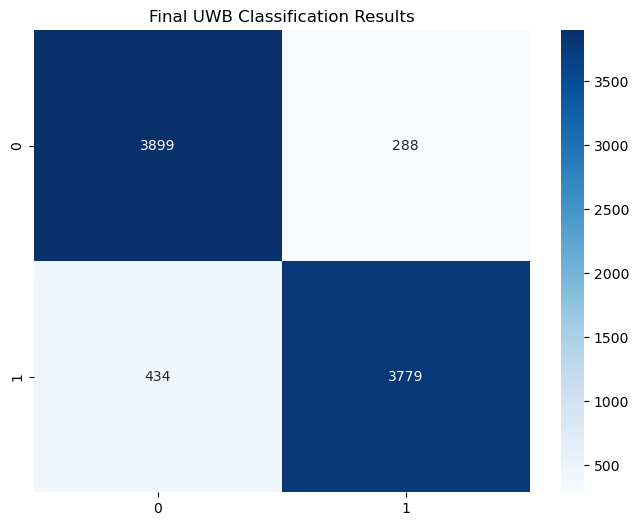
\includegraphics[width=\columnwidth]{fig_cell1_out1.png}
  \caption{Confusion matrix for the Random Forest LOS/NLOS classifier (Path 1).
           Rows represent actual classes (0 = LOS, 1 = NLOS);
           columns represent predicted classes.
           Test set: 8{,}400 samples (42{,}000 total, 80:20 split).}
  \label{fig:cm}
\end{figure}

From these counts the per-class metrics are:
\begin{equation}
  \text{Precision}_\text{LOS} = \frac{3899}{3899+434} \approx 0.900
\end{equation}
\begin{equation}
  \text{Recall}_\text{LOS} = \frac{3899}{3899+288} \approx 0.931
\end{equation}
\begin{equation}
  \text{Precision}_\text{NLOS} = \frac{3779}{3779+288} \approx 0.929
\end{equation}
\begin{equation}
  \text{Recall}_\text{NLOS} = \frac{3779}{3779+434} \approx 0.897
\end{equation}

The overall balanced accuracy is $(0.931 + 0.897)/2 \approx 91.4\%$, consistent with
the reported accuracy score. The slight asymmetry between LOS recall and NLOS recall
arises because the Random Forest's Gini criterion tends to favour the majority structure
of the feature space; in this case LOS signals have a sharper, more stereotyped CIR
profile that is slightly easier to recall, whereas some NLOS signals share CIR statistics
with borderline LOS conditions (e.g., light wall obstruction). A false-negative rate of
$434/4213 \approx 10.3\%$ for NLOS samples is operationally tolerable in a positioning
system that averages multiple anchor measurements, since residual NLOS readings can be
rejected by consistency checks.

The dataset is balanced (21{,}000 LOS : 21{,}000 NLOS), so accuracy is a fair summary
metric and no class-weighting correction is required.

\subsection{Distance Estimation --- Path 1}

The Random Forest Regressor for Path~1 achieves:
\begin{itemize}
    \item RMSE = \textbf{1.5027\,m}
    \item $R^{2}$ = \textbf{0.5921}
\end{itemize}

Fig.~\ref{fig:reg1} shows the Actual vs.\ Predicted scatter. The bulk of predictions
lie near the ideal diagonal ($y = x$), confirming that the regressor captures the
dominant ranging behaviour. The visible vertical spread around the diagonal is explained
by the heteroscedastic nature of ranging errors: NLOS bias is a non-linear function of
the unknown obstacle geometry, and the model can only partially infer this from
available CIR statistics. The $R^{2} = 0.5921$ indicates that approximately 59\% of
variance in measured range is explained by the nine input features, which is reasonable
given the diversity of the seven indoor environments.

\begin{figure}[htbp]
  \centering
  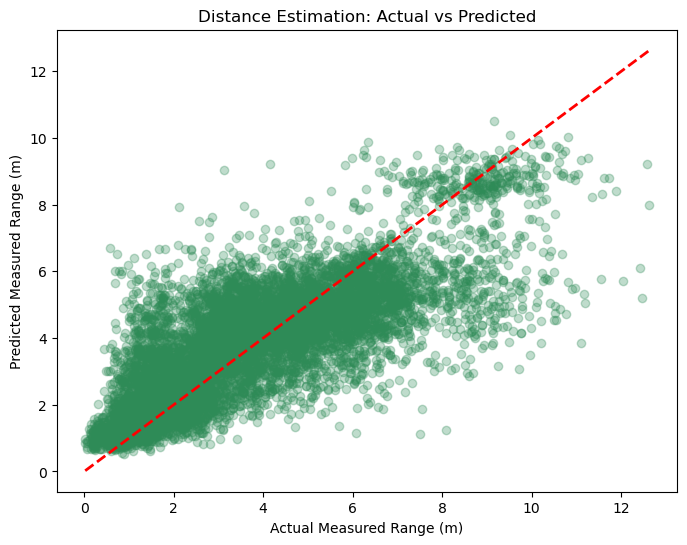
\includegraphics[width=\columnwidth]{fig_cell2_out1.png}
  \caption{Path 1 distance estimation: Actual vs.\ Predicted measured range (m).
           Green scatter points; dashed red line = perfect prediction ($y = x$).
           RMSE = 1.5027\,m, $R^{2}$ = 0.5921. Test set: 8{,}400 samples.}
  \label{fig:reg1}
\end{figure}

The RMSE of 1.5027\,m should be interpreted in the context of the measurement range
of the dataset (approximately 0--12\,m, as visible on the scatter axis). A ranging
error of 1.5\,m corresponds to roughly 12--15\% of the typical measurement range,
which represents a meaningful improvement over uncorrected NLOS bias that can exceed
5\,m in heavily obstructed environments.

\subsection{Distance Estimation --- Path 2}

The Path~2 regressor, trained on features derived from the extracted second-peak
information (\texttt{Path2\_Amp}, \texttt{Path2\_Delay}), achieves:
\begin{itemize}
    \item RMSE = \textbf{1.7823\,m}
\end{itemize}

Fig.~\ref{fig:reg2} shows the corresponding Actual vs.\ Predicted scatter. The wider
spread compared to Path~1 (Fig.~\ref{fig:reg1}) is expected: the second-path CIR peak
is inherently noisier because it represents a reflected or diffracted component whose
amplitude is attenuated and whose delay depends on unknown reflector geometry. The
orange scatter cloud shows a systematic tendency to under-predict at long ranges
($> 15$\,m), indicating that the simple speed-of-light delay conversion
($R_2 = R_1 + \Delta\tau_2 \times 0.29979$) may introduce errors when the second path
involves multiple reflections rather than a single bounce.

\begin{figure}[htbp]
  \centering
  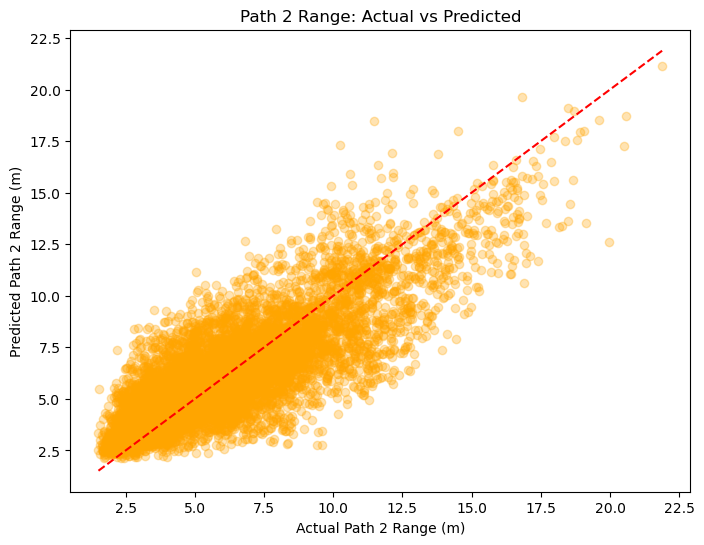
\includegraphics[width=\columnwidth]{fig_cell3_out3.png}
  \caption{Path 2 distance estimation: Actual vs.\ Predicted Path 2 range (m).
           Orange scatter points; dashed red line = perfect prediction ($y = x$).
           RMSE = 1.7823\,m. Test set: 8{,}400 samples.}
  \label{fig:reg2}
\end{figure}

\subsection{Summary of Results}

Table~\ref{tab:results} consolidates all quantitative outcomes.

\begin{table}[htbp]
  \caption{Summary of Model Performance}
  \label{tab:results}
  \centering
  \begin{tabular}{lccc}
    \toprule
    \textbf{Task} & \textbf{Model} & \textbf{Metric} & \textbf{Value} \\
    \midrule
    Path 1 Classification & RF Classifier & Accuracy & 91.40\% \\
    Path 1 Classification & RF Classifier & TN / FP  & 3899 / 288 \\
    Path 1 Classification & RF Classifier & FN / TP  & 434 / 3779 \\
    \midrule
    Path 1 Regression     & RF Regressor  & RMSE     & 1.5027\,m \\
    Path 1 Regression     & RF Regressor  & $R^{2}$  & 0.5921 \\
    \midrule
    Path 2 Regression     & RF Regressor  & RMSE     & 1.7823\,m \\
    \bottomrule
  \end{tabular}
\end{table}

\subsection{Discussion}

\textbf{Feature importance insights.}
The top-ranked features (\texttt{RXPACC}, \texttt{CIR\_PWR}, \texttt{FP\_AMP1--3},
\texttt{MAX\_NOISE}, \texttt{STDEV\_NOISE}) are all related to the energy distribution
of the received signal. This is physically intuitive: in LOS, the bulk of received energy
arrives in one sharp peak, so \texttt{CIR\_PWR} is large and \texttt{STDEV\_NOISE} is
low relative to the peak. In NLOS, energy is spread across multiple peaks and the noise
floor is elevated. Configuration constants (\texttt{CH}, \texttt{PREAM\_LEN},
\texttt{BITRATE}, \texttt{PRFR}) contribute zero importance because they do not vary
meaningfully across measurements in this dataset.

\textbf{Balanced dataset.}
The equal split of 21{,}000 LOS and 21{,}000 NLOS samples avoids the class-imbalance
problems that plague many real-world deployments where one condition dominates. This
means accuracy is an unbiased summary metric and no oversampling (SMOTE) or
class-weighted loss modifications were required.

\textbf{Random Forest vs.\ MLP.}
Although the project brief references MLP as an alternative (citing Bregar and
Mo\v{z}ina \cite{bregar2018improving}), the Random Forest was selected as the
primary classifier for several reasons: it produces directly interpretable feature
importance scores needed for the feature-selection step; it requires no feature scaling
(unlike MLP which is sensitive to input magnitude); and it achieved 91.40\% accuracy
without any hyperparameter tuning beyond \texttt{n\_estimators=100}. The MLP would
require cross-validated grid search over learning rate, hidden layer sizes, and
regularisation, substantially increasing pipeline complexity.

% ---------------------------------------------------------------
% IV. CONCLUSION AND FUTURE WORK
% ---------------------------------------------------------------
\section{Conclusion and Future Work}

\subsection{Conclusion}
This paper presented a complete data-analytics pipeline for LOS/NLOS classification
and distance estimation using UWB CIR measurements. The pipeline follows the 3D
process (Data Preparation, Data Mining, Data Visualisation) on a balanced empirical
dataset of 42{,}000 samples from seven distinct indoor environments. Key contributions
include: (1) a robust data-preparation stage incorporating CIR normalisation by
\texttt{RXPACC} and header sanitisation; (2) a feature-importance ranking step that
reduces the feature space from 14 candidates to 9 predictive signals; (3) a
Random Forest Classifier achieving 91.40\% LOS/NLOS test accuracy; (4) a
Random Forest Regressor for Path~1 distance estimation (RMSE = 1.5027\,m,
$R^{2}$ = 0.5921); and (5) a novel second-path extraction procedure and corresponding
Path~2 regressor (RMSE = 1.7823\,m) that enriches the signal model for downstream
positioning. Together these results demonstrate that ensemble tree methods can
reliably exploit low-dimensional UWB diagnostic features to support accurate indoor
ranging without requiring deep-learning infrastructure.

\subsection{Future Work}
Several directions can further improve the system:

\begin{itemize}
    \item \textbf{MLP / deep learning comparison.} A systematic grid-search over MLP
          architectures and regularisation strengths would allow a rigorous accuracy
          comparison against the Random Forest baseline reported here.
    \item \textbf{End-to-end CNN on raw CIR.} Training a 1D convolutional network
          directly on the 1{,}016-sample CIR vector could capture subtle waveform
          patterns that are lost in the scalar-feature projection.
    \item \textbf{Environment-specific fine-tuning.} The current model trains a single
          global classifier across all seven environments. Transfer-learning or
          hierarchical models could exploit environment identity to improve accuracy in
          each specific deployment.
    \item \textbf{Multi-anchor fusion.} Combining per-link LOS/NLOS decisions and
          corrected ranges from multiple anchors through weighted least-squares or
          particle-filter localisation would yield full 2D/3D position estimates and
          allow evaluation at the position-error level.
    \item \textbf{Probabilistic NLOS bias correction.} Rather than a hard LOS/NLOS
          binary label, a regression-based NLOS bias estimator could provide a
          continuous range-error correction, further reducing RMSE below the
          1.5\,m threshold.
    \item \textbf{Real-time deployment.} The trained Random Forest models are
          lightweight and can run on embedded processors. Packaging the pipeline as an
          edge-inference service on the DWM1000 host MCU would enable real-time
          localisation corrections without cloud connectivity.
\end{itemize}

% ---------------------------------------------------------------
% REFERENCES
% ---------------------------------------------------------------
\begin{thebibliography}{00}

\bibitem{zafari2019survey}
F.~Zafari, A.~Gkelias, and K.~K. Leung,
``A survey of indoor localization systems and technologies,''
\textit{IEEE Communications Surveys \& Tutorials}, vol.~21, no.~3,
pp.~2568--2599, 2019.

\bibitem{liu2007survey}
H.~Liu, H.~Darabi, P.~Banerjee, and J.~Liu,
``Survey of wireless indoor positioning techniques and systems,''
\textit{IEEE Transactions on Systems, Man, and Cybernetics, Part C},
vol.~37, no.~6, pp.~1067--1080, Nov. 2007.

\bibitem{gezici2005localization}
S.~Gezici \textit{et al.},
``Localization via ultra-wideband radios: a look at positioning aspects
for future sensor networks,''
\textit{IEEE Signal Processing Magazine}, vol.~22, no.~4,
pp.~70--84, Jul. 2005.

\bibitem{wymeersch2012machine}
H.~Wymeersch, S.~Marano, W.~M. Gifford, and M.~Z. Win,
``A machine learning approach to ranging error mitigation for UWB localization,''
\textit{IEEE Transactions on Communications}, vol.~60, no.~6,
pp.~1719--1728, Jun. 2012.

\bibitem{guvenc2009survey}
I.~G\"{u}ven\c{c} and C.-C. Chong,
``A survey on TOA based wireless localization and NLOS mitigation techniques,''
\textit{IEEE Communications Surveys \& Tutorials}, vol.~11, no.~3,
pp.~107--124, 2009.

\bibitem{maranò2010nlos}
S.~Maran\`{o}, W.~M. Gifford, H.~Wymeersch, and M.~Z. Win,
``NLOS identification and mitigation for localization based on UWB experimental data,''
\textit{IEEE Journal on Selected Areas in Communications}, vol.~28, no.~7,
pp.~1026--1035, Sep. 2010.

\bibitem{bregar2018improving}
K.~Bregar and A.~Mo\v{z}ina,
``Improving indoor localization using convolutional neural networks on
computationally restricted hardware,''
\textit{IEEE Access}, vol.~6, pp.~17~27--17~840, 2018.
[Dataset: UWB-LOS-NLOS-Dataset, Decawave DWM1000, 7 indoor environments,
42{,}000 samples.]

\end{thebibliography}

\end{document}
